\documentclass[10pt]{beamer}

\usetheme[progressbar=frametitle]{metropolis}
\usepackage{appendixnumberbeamer}
\usepackage{graphicx} % Required for inserting images
\graphicspath{ {./Photos/} }
\usepackage{booktabs}
\usepackage[scale=2]{ccicons}
\usepackage[font={scriptsize,it}]{caption}
\usepackage{pgfplots}
\usepgfplotslibrary{dateplot}
\setbeamercolor{block body alerted}{bg=alerted text.fg!10}
\setbeamercolor{block title alerted}{bg=alerted text.fg!20}
\setbeamercolor{block body}{bg=structure!10}
\setbeamercolor{block title}{bg=structure!20}
\setbeamercolor{block body example}{bg=green!10}
\setbeamercolor{block title example}{bg=green!20}

\usepackage{xspace}
\newcommand{\themename}{\textbf{\textsc{metropolis}}\xspace}

\title{Monuments at UNC-Chapel Hill}

% \date{\today}
\date{May 2024}
\author{Andrew Ye}


\begin{document}


\frame{\titlepage}

\begin{frame}
\frametitle{Table of Contents}
\setbeamertemplate{section in toc}[sections numbered]
\tableofcontents
\end{frame}

\section{Monuments}

\begin{frame}{Silent Sam(1913 - 2018)}
    \begin{minipage}{0.5\textwidth}
    \begin{figure}
        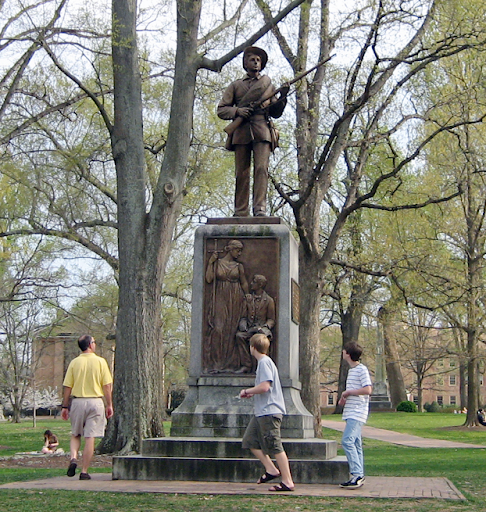
\includegraphics[scale = 0.3]{photos/photo1.png}
    \end{figure}
    \end{minipage}
    \begin{minipage}{0.4\textwidth}
    \begin{figure}
        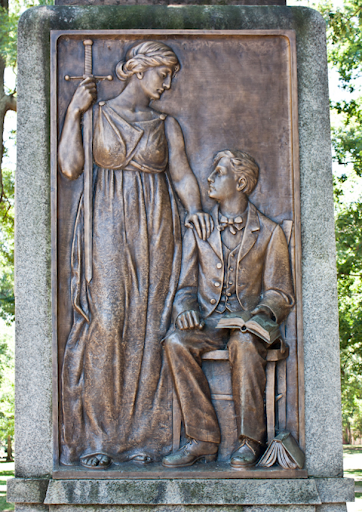
\includegraphics[scale = 0.3]{photos/photo4.png}
    \end{figure}
    \end{minipage}
\end{frame}
\begin{frame}{Silent Sam(1913 - 2018)}
    \begin{minipage}{0.5\textwidth}
    \begin{figure}
        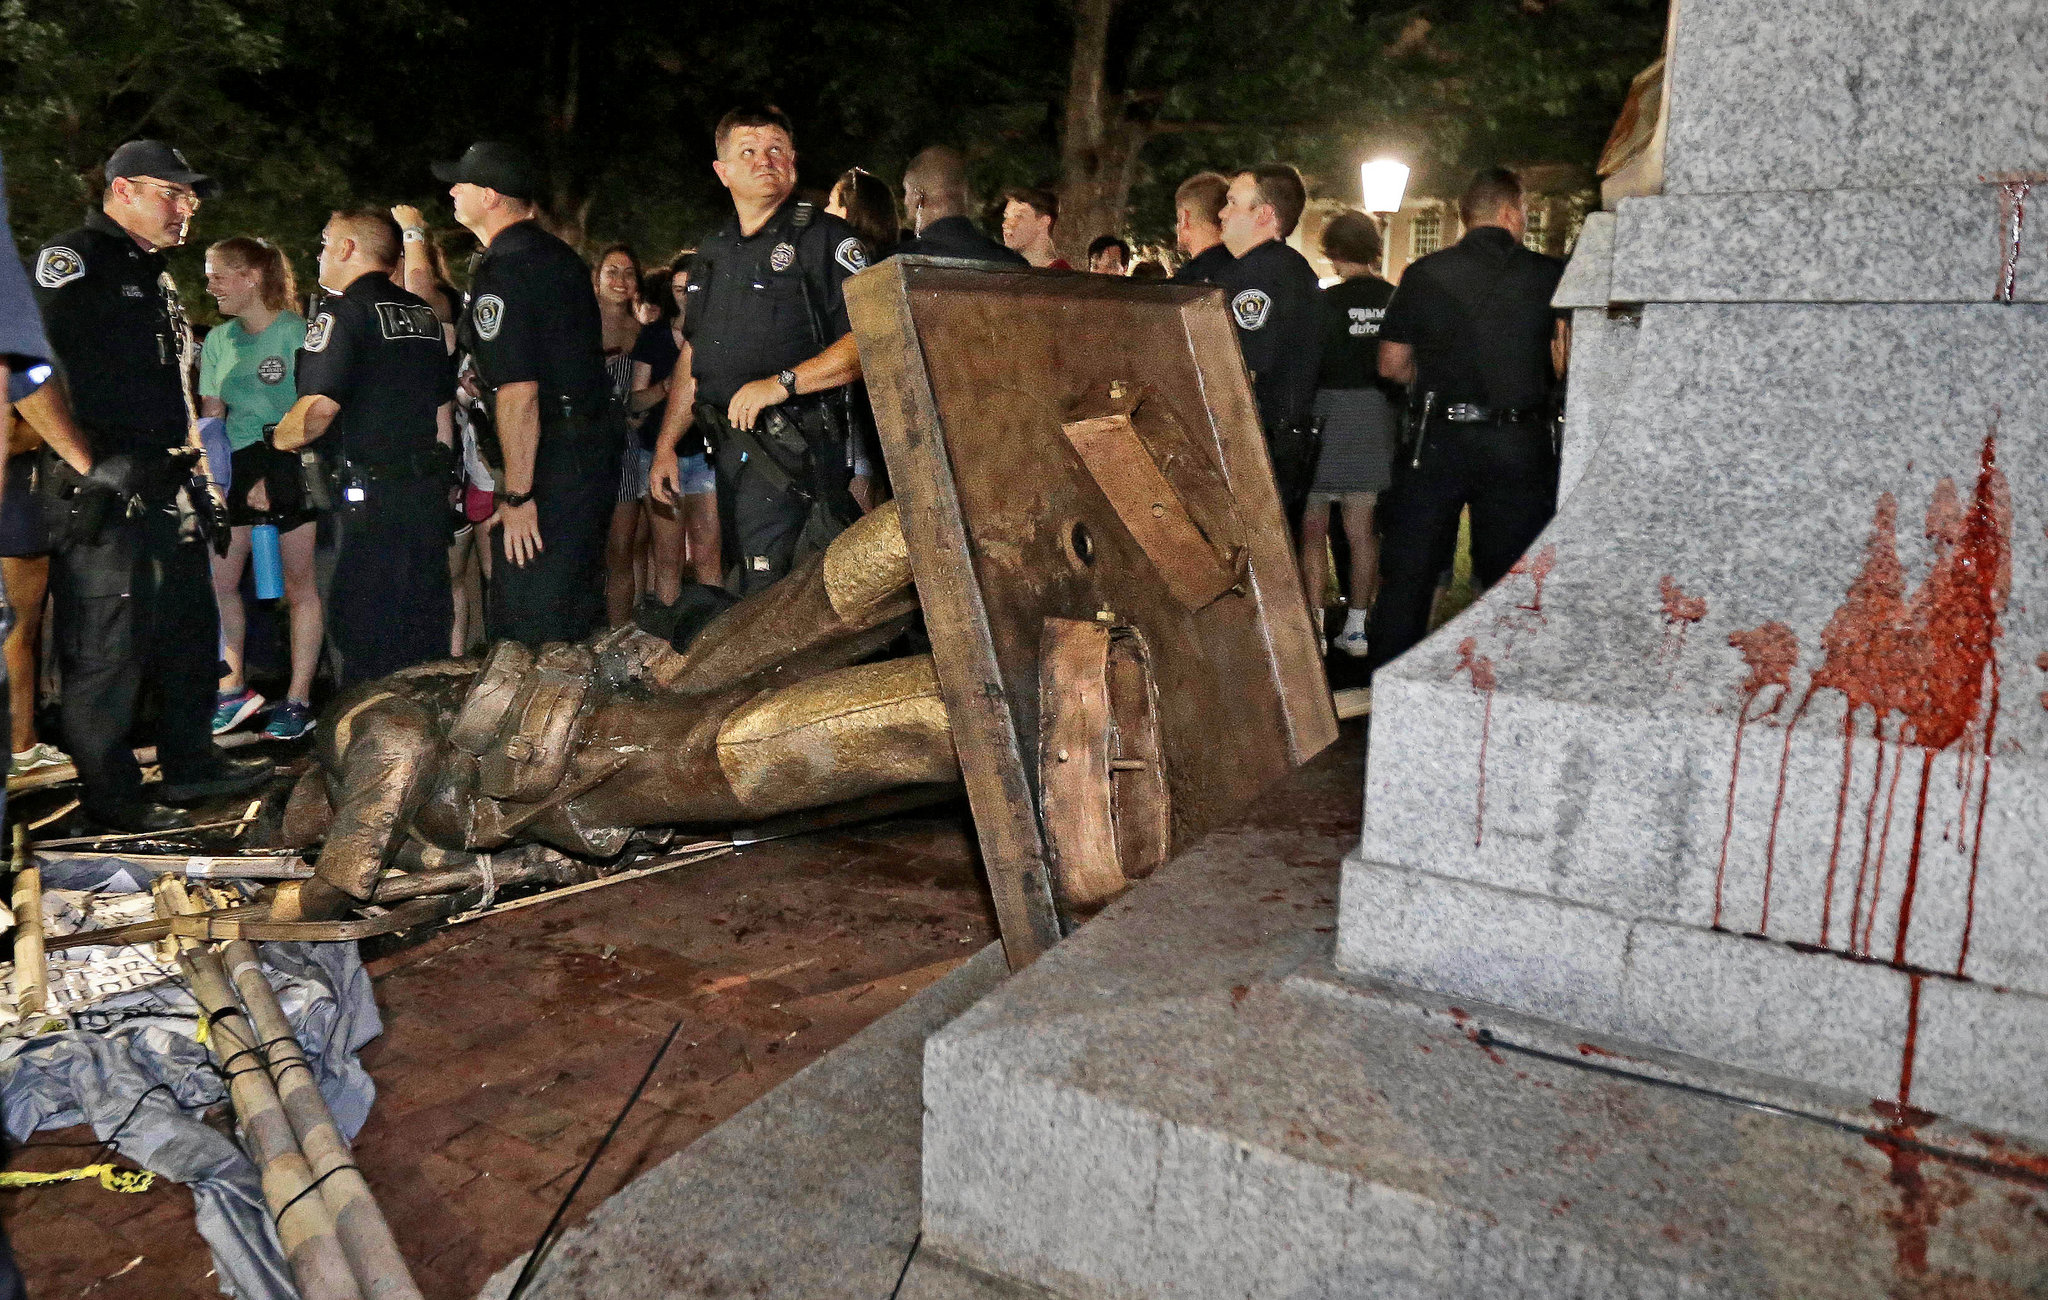
\includegraphics[scale = 0.3]{photos/photo6.jpg}
        \caption{August 2018}
    \end{figure}
    \end{minipage}
    \begin{minipage}{0.4\textwidth}
    \begin{figure}
        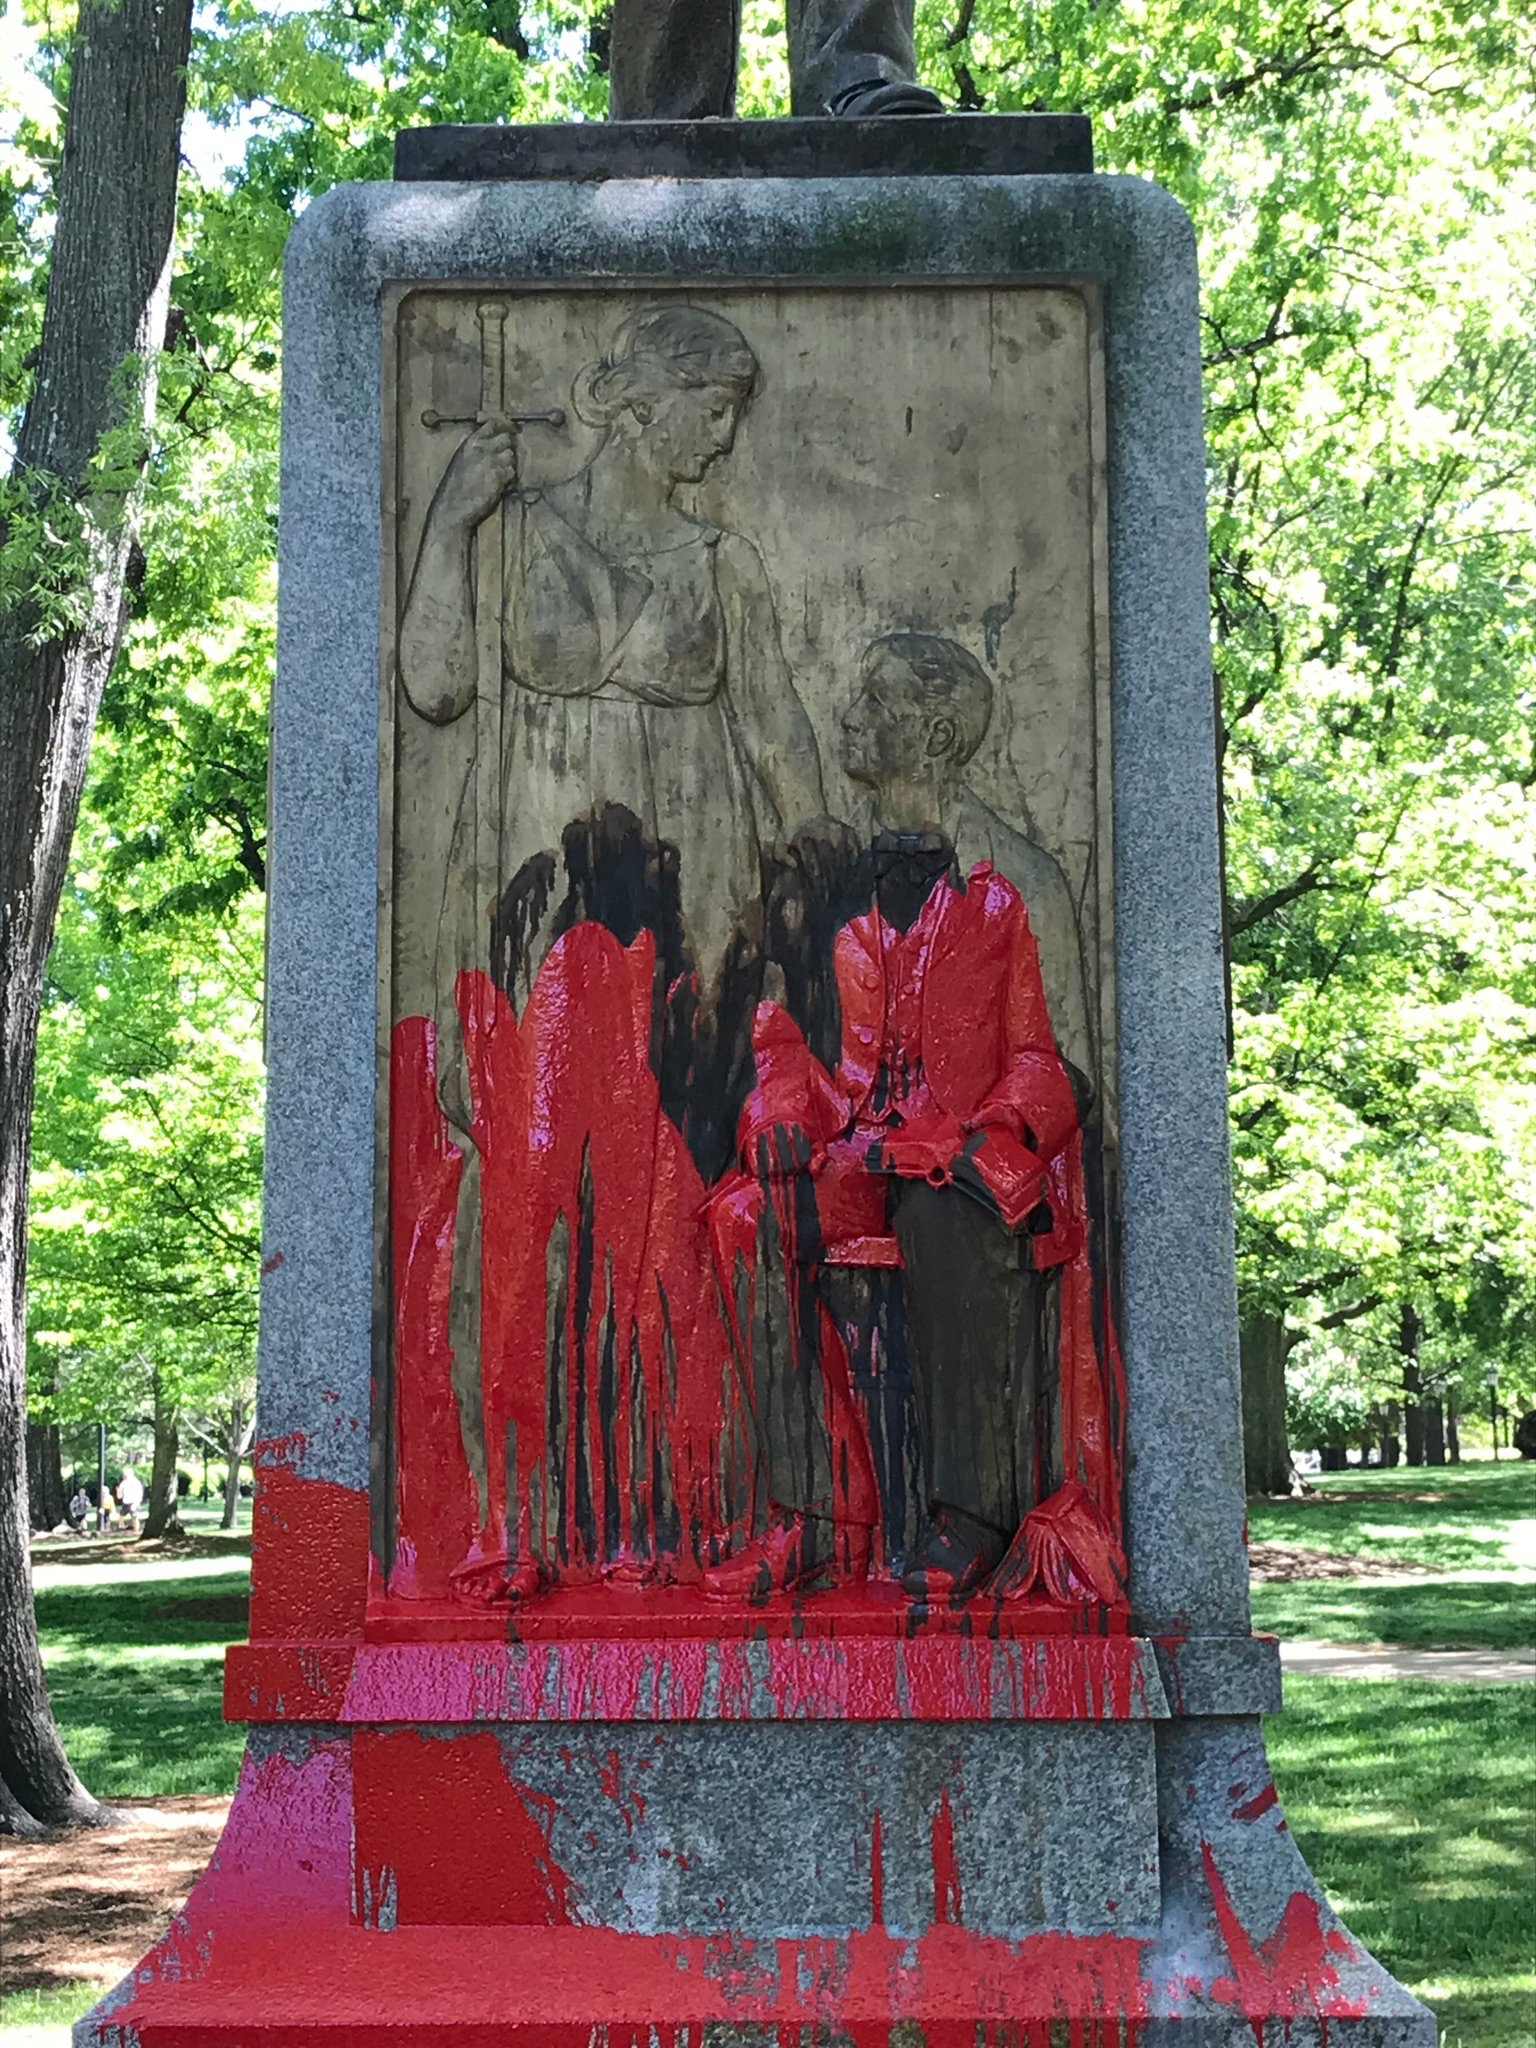
\includegraphics[scale = 0.09]{photos/photo7.JPG}
        \caption{April 2018}
    \end{figure}
    \end{minipage}
\end{frame}

\begin{frame}{Unsung Founders, Bond and Free(2005-Present)}
    \begin{minipage}{0.5\textwidth}
    \begin{figure}
        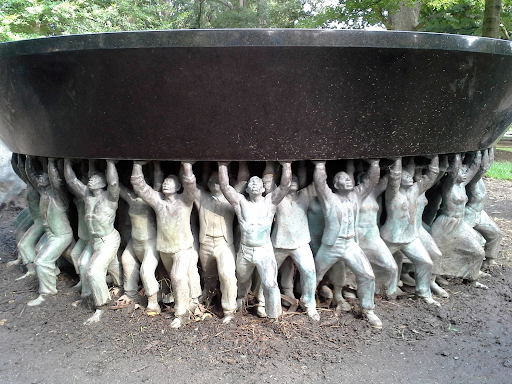
\includegraphics[scale = 0.3]{photos/photo2.png}
    \end{figure}
    \end{minipage}
    \begin{minipage}{0.4\textwidth}
   
    \begin{figure}
        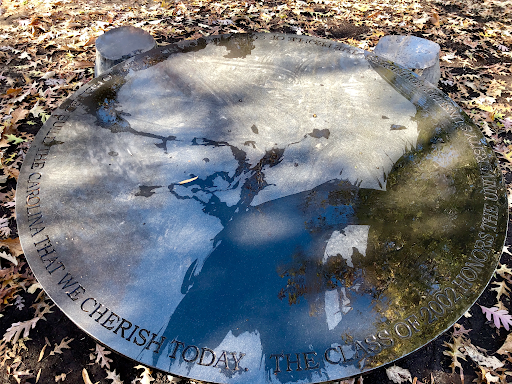
\includegraphics[scale = 0.3]{photos/photo3.png}
        \caption{ “The class of 2002 honors the university’s unsung founders – the people of color, bond and free – who helped build the Carolina that we cherish today.”}
    \end{figure}
     \vspace{-2.4cm}
    \end{minipage}
\end{frame}
\begin{frame}{Unsung Founders, Bond and Free(2005-Present)}
\begin{figure}
\centering
    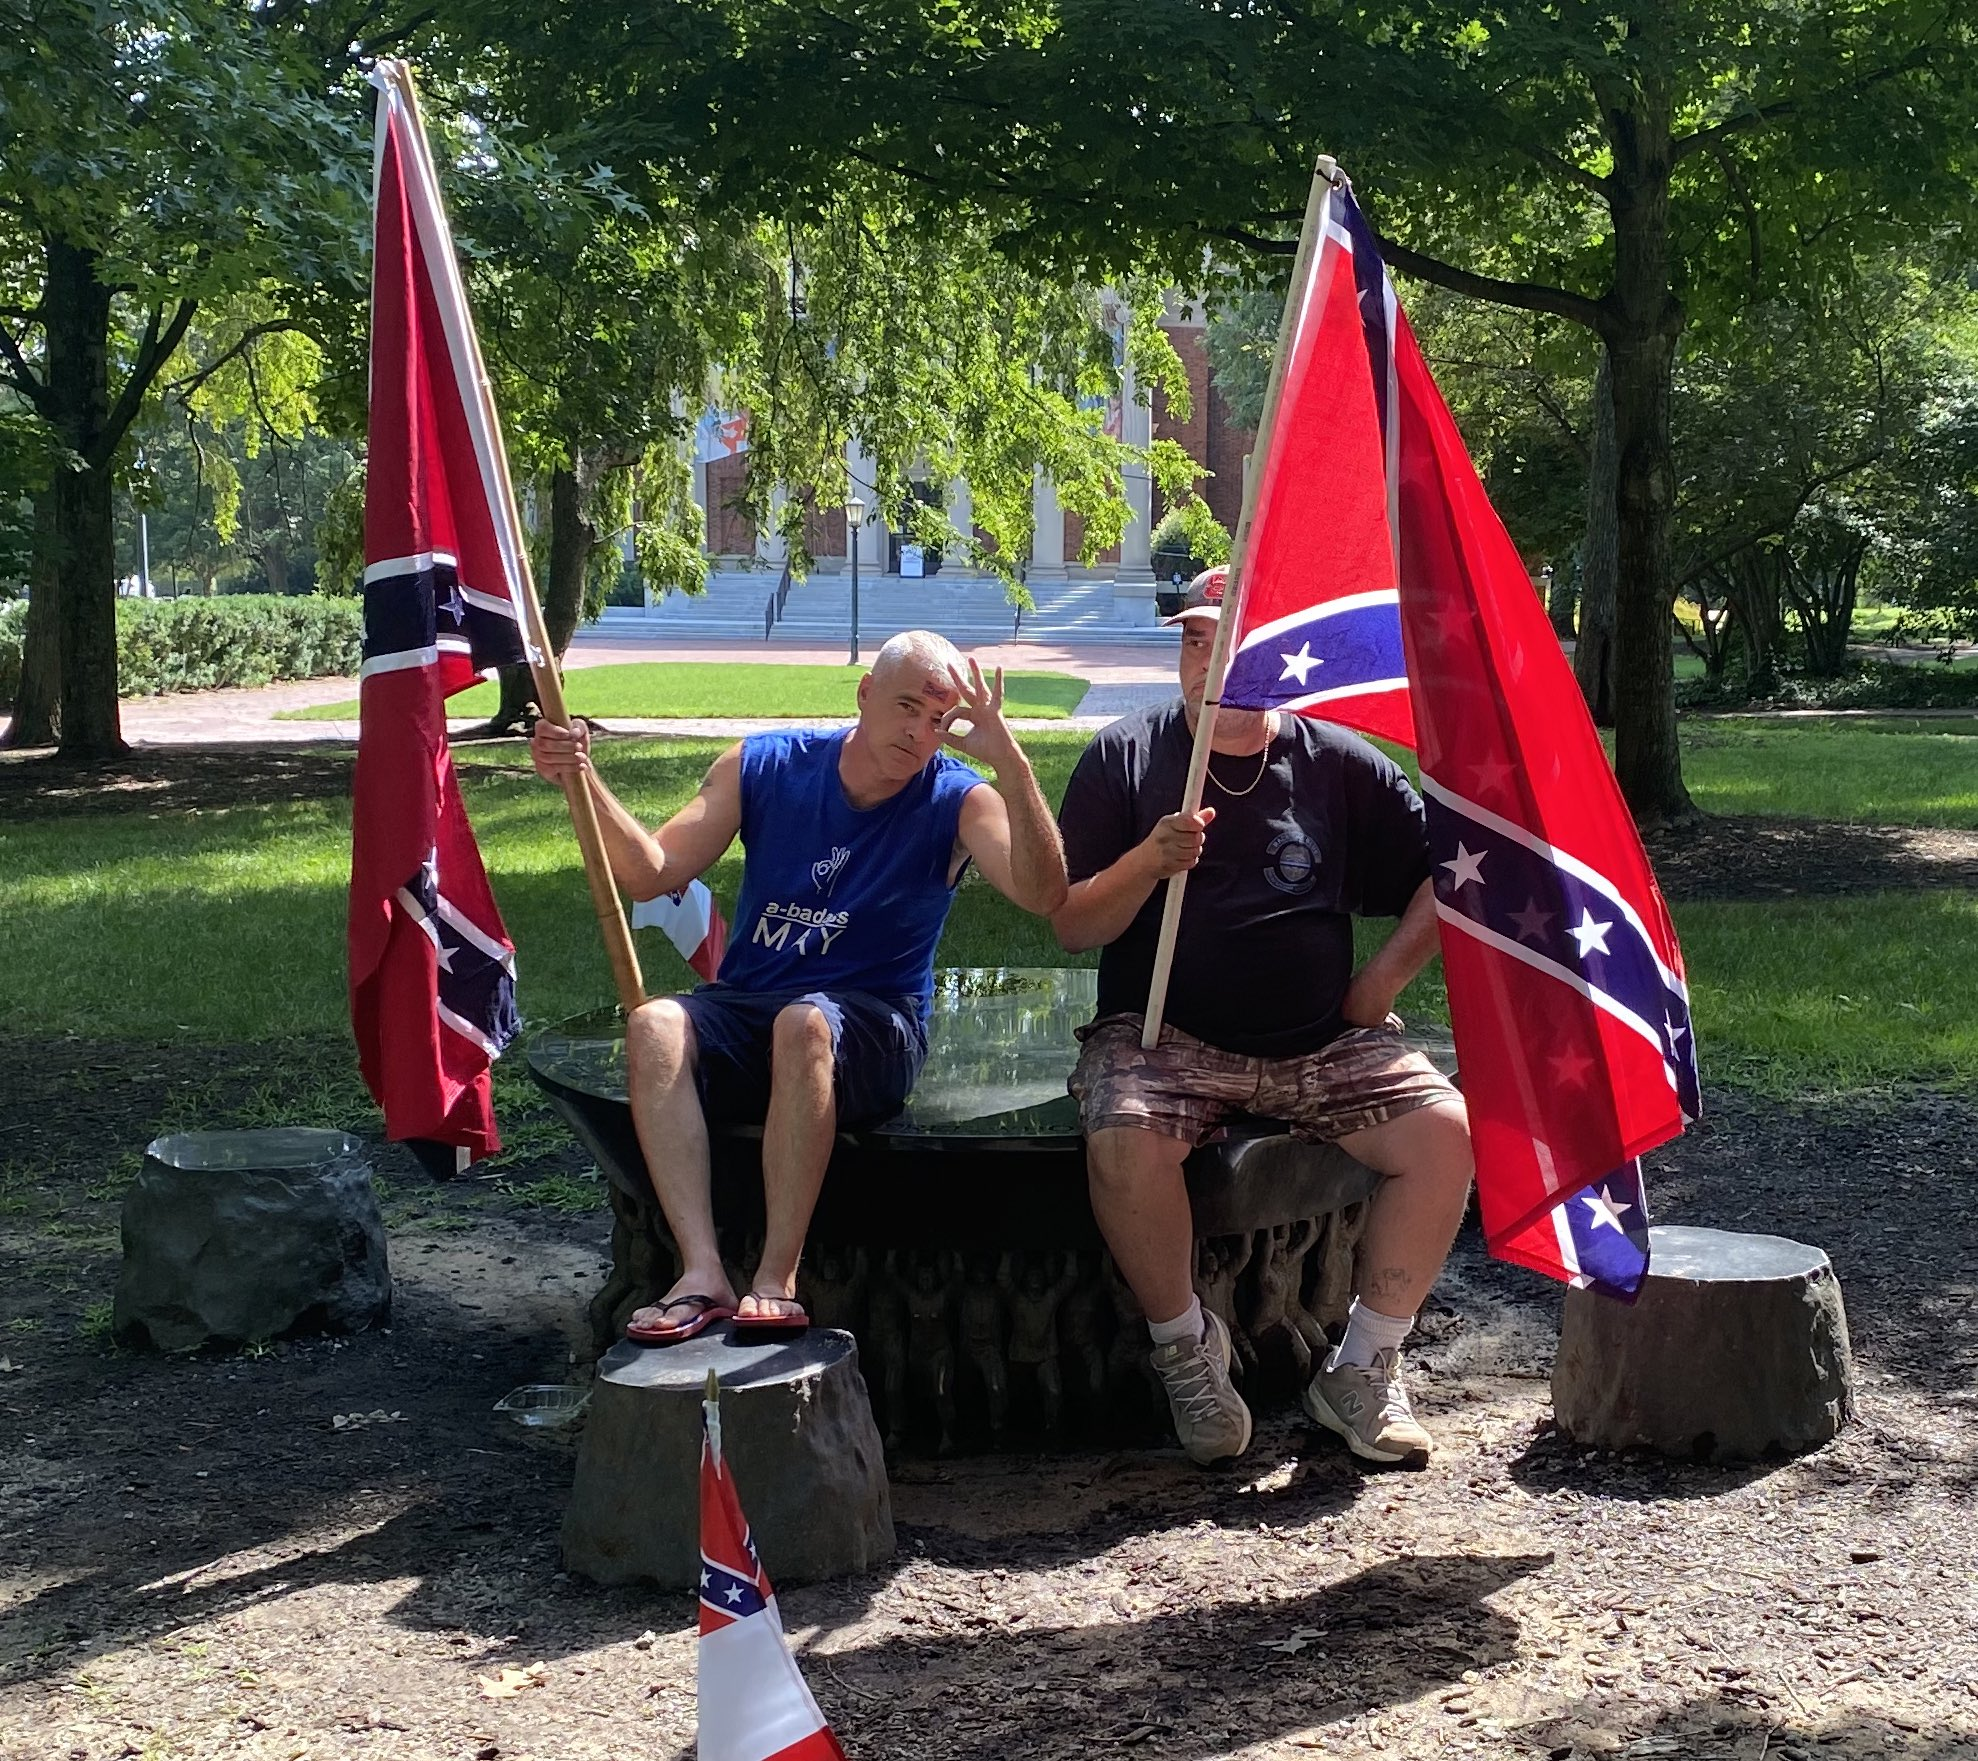
\includegraphics[scale = 0.1]{photos/photo8.jpg}
    \caption{July 2021}
\end{figure}
\end{frame}


\section{Remembering History}
\begin{frame}{Remembering History}
    \begin{alertblock}{Events in Time vs History}
        Note the difference between what happened at a certain point in time, in which there is one version, and history, a changing narrative. 
    \end{alertblock}
    The two monuments tell a different narrative about Chapel Hill.
\end{frame}

\begin{frame}{Narrative of Silent Sam}
    \begin{minipage}{0.5\textwidth}
    \begin{itemize}
        \item Defenders of the statue believe that there is one history that should be preserved. 
        \item The lens that the \textit{Silent Sam} statue represents       is one that glorifies the Confederacy and white supremacy.
    \end{itemize}
    \end{minipage}
    \begin{minipage}{0.4\textwidth}
        \begin{figure}
            \centering
            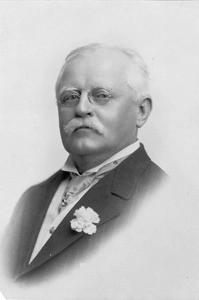
\includegraphics[scale = 2]{photos/photo5.jpg}
            \caption{``Their courage and steadfastness saved the very life of the Anglo Saxon race in the South.'' \\ - Julian Carr}
        \end{figure}
    \end{minipage}
\end{frame}

\begin{frame}{Narrative of Unsung Founders}
    \begin{minipage}{0.5\textwidth}
        \begin{itemize}
            \item Intended to honor the enslaved individuals in Chapel Hill who helped construct UNC and the town around it.
            \item Criticism of monument regarding its effectiveness and message. 
        \end{itemize}
    \end{minipage}
    \begin{minipage}{0.4\textwidth}
   
    \begin{figure}
        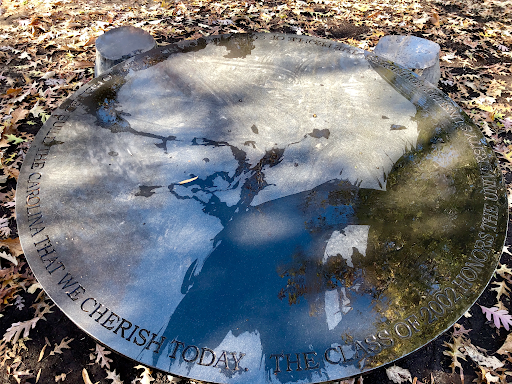
\includegraphics[scale = 0.3]{photos/photo3.png}
        \caption{ “The class of 2002 honors the university’s unsung founders – the people of color, bond and free – who helped build the Carolina that we cherish today.”}
    \end{figure}
     \vspace{-2.4cm}
    \end{minipage}
\end{frame}



\begin{frame}{}
  \centering \Large
  \emph{Thank You}
\end{frame}


\end{document}
